% ===================================================================
% Preprint Title: A 3D Mathematical Model of a Dynamically Coupled Field...
% Author: Toshiya Konno
% Version: 5.0 (Final Manuscript) (Date: 2025-07-30)
% This is the definitive final version, incorporating all reviewer points,
% supplementary experiments, theoretical refinements, and final polishing.
% ===================================================================

\documentclass[a4paper,11pt,ja=standard,lualatex]{bxjsarticle}

% ---------- Packages ----------
\usepackage{fontspec}
\usepackage{amsmath,amssymb,amsfonts}
\usepackage{graphicx}
\usepackage{geometry}
\usepackage{hyperref}
\usepackage{authblk}
\usepackage{placeins}
\usepackage{caption}
\usepackage{unicode-math} 

% ---------- PDF Metadata (Final for v5.0) ----------
\hypersetup{
  pdftitle={A 3D Mathematical Model of a Dynamically Coupled Field Inspired by Operator Algebras (Version 5.0)},
  pdfauthor={Toshiya Konno},
  pdfsubject={This paper quantitatively demonstrates the existence and universality of stochastic resonance in our model through extensive numerical simulations and provides a theoretical explanation for the observed phase structure based on linear stability analysis.},
  pdfkeywords={Coupled Gross–Pitaevskii Equations; Quantum-Classical Hybrid System; Stochastic Resonance; Phase Diagram; Universality; Linear Stability Analysis; Dissipation; Thermal Fluctuation},
  pdfcreator={XeLaTeX (TeX Live)},
  pdflang={en}
}

% ---------- Fonts & Math Fonts ----------
\setmainfont{TeX Gyre Termes}
\setjamainfont{IPAexMincho}
\setsansfont{IPAexGothic}
\setmathfont{TeX Gyre Termes Math}
\renewcommand{\sfdefault}{IPAexGothic}
\newfontfamily\dejavusans{TeX Gyre Termes}
\newfontfamily\liberationsans{TeX Gyre Termes}

% ---------- Layout ----------
\geometry{left=25mm,right=25mm,top=25mm,bottom=25mm}

% ---------- Title, Author, Date (Final for v5.0) ----------
\title{作用素環論に着想を得た動的結合場の3次元数式モデル\\
\large A 3D Mathematical Model of a Dynamically Coupled Field Inspired by Operator Algebras: Theoretical Foundation and Numerical Verification of Stable Coupled Motion}
\author[1]{今野聖也\,Toshiya Konno}
\affil[1]{Independent Researcher\\\href{mailto:ktlifeisonlyreallyoverafter60@gmail.com}{ktlifeisonlyreallyoverafter60@gmail.com}}
\date{2025年7月30日(Version 5.0)}

\begin{document}
\maketitle

\noindent\textbf{Keywords:}\ Coupled Gross–Pitaevskii Equations; Quantum-Classical Hybrid System; Tensegrity; Soliton Dynamics; Topological Robustness; Operator Algebras; Dissipation; Phase Transition; Thermal Fluctuation; Stochastic Resonance; Universality; Linear Stability Analysis

% ---------- Abstract (Japanese - Final Version) ----------
\begin{abstract}
\noindent 以前の研究(Version 4.0)において、我々は作用素環論に着想を得た量子・古典結合系の3次元数式モデルに揺動散逸定理を導入し、「熱的励起振動状態(TEOS)」という新たな動的平衡状態と、確率共鳴の強い兆候を報告した。本稿は、その探求をさらに深化させ、系の豊かな物理現象に対する、厳密な定量的検証と、統一的な理論的説明を与えるものである。まず、大規模な数値シミュレーションを実行し、信号対雑音比(SNR)という厳密な指標を用いて、確率共鳴の存在を統計的に有意な形で定量的に示す。さらに、散逸係数を変化させた複数の条件下でもこの現象が普遍的に観測されることを明らかにし、散逸が確率共鳴の増幅効果に与える影響についての、新たな知見を提示する。これらの数値計算結果を補完するため、我々は、系の運動方程式の線形安定性解析に基づいた、新たな理論的枠組みを構築した。この理論は、観測された3つの相(安定結合移動、固定状態、TEOS)の構造を支配する相図の境界線を、第一原理から導出する。これらの数値的検証と理論的考察の組み合わせは、我々のモデルの物理的妥当性を確固たるものにするだけでなく、複雑な系が、いかにしてノイズを利用して頑健な情報伝達を達成しうるかという、生命現象にも通じる根源的な問いに対して、深く、そして新しい洞察を提供する。
\end{abstract}

% ---------- Abstract (English - Final Version) ----------
\vspace{1em}
\noindent\textbf{Abstract}
\par\noindent
\small
In our previous work (Version 4.0), we introduced thermal fluctuations into our 3D mathematical model of a dynamically coupled quantum-classical system, revealing a novel "Thermally Excited Oscillatory State" (TEOS) and strong indications of stochastic resonance (SR). This paper builds directly upon that foundation, presenting a rigorous quantitative and theoretical analysis of the system's rich phenomenology. Through extensive numerical simulations, performing a large number of runs to ensure statistical reliability, we quantitatively demonstrate the existence of SR by analyzing the signal-to-noise ratio (SNR), identifying an optimal noise intensity that maximizes signal amplification. Furthermore, we show the universality of this phenomenon across a range of dissipation strengths, providing new insights into the interplay between dissipation and the effectiveness of SR. Complementing these numerical results, we develop a theoretical framework based on linear stability analysis. This framework explains the structure of the system's phase diagram—comprising the stable coupled, pinned, and TEOS phases—by deriving the critical conditions for phase transitions from first principles. These combined findings not only solidify the physical relevance of our model but also provide a deeper, mechanistic understanding of how complex systems can harness noise for robust information transport, offering a potential physical framework for understanding robust information transport in complex, noisy environments. These mechanisms are akin to those found in intracellular processes.
\normalsize
\vspace{2em}

\FloatBarrier
% ... (中略: 導入から結論までの本文は、ご提供いただいた最終稿と同一です) ...
\section{導入 (Introduction)}
生命の基本単位である細胞は、その内部において、熱揺らぎや粘性による散逸が支配的な環境下にありながら、驚くほど効率的で、かつ正確な情報伝達を行っている。このようなノイズの多い環境における生命現象の頑健性は、現代物理学における重要な研究テーマの一つである\cite{lindner}。この一見矛盾した現象を説明するため、我々は、作用素環論\cite{vonneumann, bratteli}の思想に基づき、量子場と古典場が動的に結合する3次元数式モデルを構築してきた。

以前の研究(v2.5, v3.0)では、理想系における「安定結合移動」と、散逸導入時の「一次相転移的な崩壊」を報告した。続く研究(v4.0)では、揺動散逸定理に基づき系に熱ゆらぎを導入し、散逸によるエネルギー損失を熱浴からのエネルギー注入で補う、新たな動的平衡状態「熱的励起振動状態(TEOS)」の存在を明らかにした。さらに、このTEOSにおいて、熱ゆらぎが量子場からの微弱な信号を増幅する「確率共鳴(Stochastic Resonance, SR)」\cite{benzi, mcnamara, gammaitoni}の強い兆候を観測した。

本稿は、v4.0で残された課題に答えるものである。我々は、(1) 大規模な数値シミュレーションを通じて、信号対雑音比(SNR)という厳密な指標を用い、確率共鳴の存在を統計的に有意な形で定量的に検証し、その普遍性を明らかにする。そして、(2) 系の支配方程式の線形安定性解析に基づいた理論的枠組みを構築し、観測された相構造の起源を、第一原理から説明する。この数値的「証拠」と理論的「証明」の組み合わせを通じて、我々のモデルが、生命現象にも通じる、ノイズを利用した情報伝達の本質的な物理メカニズムを、いかに捉えているかを、深く論じる。

\FloatBarrier
\section{モデル本体 (The Model)}
本研究で用いる数式モデルの基本構造は、以前の研究(v3.0, v4.0)で提示したものと同一である。本モデルは、作用素環論の思想に基づき、量子場と古典場がヘルマン-ファインマン力と自己復元力を介して結合する、自己無撞着な系として構築される。

\subsection{基本方程式系 (Fundamental Equations)}
本モデルは、量子場 $\psi(\mathbf{r},t)$(GP波動関数)と、1自由度の古典場 $u(t)$(障壁の中心位置 $z_b(t)$)の動的な相互作用を記述する。古典場には、環境との相互作用をモデル化するため、散逸項と熱ゆらぎ項が含まれており、その運動はランジュバン方程式で記述される。系全体は以下の連成方程式系によって定義される。
\begin{align}
 i\hbar\frac{\partial\psi(\mathbf r,t)}{\partial t}&=H[u(t)]\psi(\mathbf r,t), \label{eq:schrodinger_v5} \\
  M\frac{d^{2}u(t)}{dt^{2}}&=F_{\text{feedback}}[\psi,u]+F_{\text{restoring}}[u] - \gamma \frac{du(t)}{dt} + F_{\text{thermal}}(t). \label{eq:langevin_v5}
\end{align}
この方程式系は、有限温度のボース・アインシュタイン凝縮体を記述するために提案されている、確率的グロス・ピタエフスキー方程式\cite{bradley}の考え方と共通の構造を持つ。(シミュレーションでは、$\hbar=1$とする無次元化単位系を用いる。)

\subsection{ハミルトニアンと力の具体的定義 (Detailed Definitions of Hamiltonian and Forces)}

\paragraph{全ハミルトニアン (Total Hamiltonian)}
\begin{equation}
    H = -\frac{\hbar^2}{2m}\nabla^2 + V_{\text{trap}}(\mathbf{r}) + V_{\text{barrier}}(\mathbf{r}, u(t)) + g|\psi|^2.
\end{equation}

\paragraph{外部ポテンシャル (External Potential)}
外部ポテンシャル $V_{\text{ext}}(\mathbf{r}, u) = V_{\text{trap}}(\mathbf{r}) + V_{\text{barrier}}(\mathbf{r}, u)$ は、量子場を横方向に閉じ込める調和トラップと、動的な障壁から構成される。
\begin{itemize}
    \item \textbf{横方向閉じ込め:} $V_{\text{trap}}(\mathbf{r}) = \frac{1}{2}m\omega_{\perp}^2(x^2+y^2)$.
    \item \textbf{動的障壁:} $V_{\text{barrier}}(\mathbf{r}, u(t)) = A \exp\left(-\frac{(z-z_b(t))^2}{2\sigma^2}\right)$.
\end{itemize}
ここで、$z_b(t)$が、我々のモデルにおける古典場の自由度 $u(t)$ である。

\paragraph{フィードバック力 (Hellmann-Feynman Force)}
\begin{equation}
    F_{\text{feedback}} = -\left\langle \psi \left| \frac{\partial H}{\partial z_b} \right| \psi \right\rangle = -\int \psi^*(\mathbf{r},t) \frac{\partial V_{\text{barrier}}}{\partial z_b} \psi(\mathbf{r},t) d^3r.
\end{equation}

\paragraph{自己復元力 (Tensegrity-like Restoring Force)}
\begin{equation}
    F_{\text{restoring}} = -k_{\text{mech}}(z_b(t) - z_{b,0}).
\end{equation}
ここで、$z_{b,0}$は障壁の平衡位置(本研究では0)である。

\paragraph{非線形相互作用 (Nonlinear Interaction)}
本モデルでは、ソリトンの自己束縛を可能にするため、引力相互作用 $g < 0$ を仮定する。3次元空間における引力相互作用系の崩壊は、強い横方向閉じ込めポテンシャル $V_{\text{trap}}$ によって系が実効的に準1次元化されるため、本研究で扱った粒子数の範囲では抑制される。

\subsection{主要な記号とパラメータ (Key Symbols and Parameters)}
本研究で用いる主要な記号と、シミュレーションで標準的に用いたパラメータ値を、表\ref{tab:params}にまとめる。

\begin{table}[h!]
\centering
\caption{主要な記号とシミュレーションパラメータ。}
\begin{tabular}{l l l}
\hline
\textbf{Symbol} & \textbf{Meaning} & \textbf{Value (dimensionless)} \\
\hline
$\psi$ & Quantum field wave function & - \\
$u$ ($z_b$) & Classical field displacement & - \\
$A$ & Barrier potential amplitude & 0.1 \\
$\sigma$ & Barrier potential width & 4.0 \\
$g$ & Nonlinear interaction strength & -15.0 \\
$k_{\text{mech}}$ & Restoring force spring constant & 10.0 \\
$M$ & Effective mass of the classical field & 50.0 (Standard) \\
$k_{z,\text{kick}}$ & Initial momentum (wavenumber) & 0.15 (Standard) \\
$\gamma$ & Damping coefficient & 0.0 -- 3.0 (swept) \\
$T$ & Thermal strength (temperature) & 0.0 -- 3.0 (swept) \\
\hline
\end{tabular}
\label{tab:params}
\end{table}

\FloatBarrier
\section{結論と将来課題 (Conclusion and Future Work)}
本研究において、我々は、作用素環論に着想を得た3次元数式モデルの探求を、大きく前進させた。大規模な数値シミュレーションを通じて、確率共鳴の存在を定量的に検証し、その普遍性を明らかにした。また、線形安定性解析に基づいた理論的枠組みを構築し、観測された相構造の起源を説明した。

我々の結果は、本モデルが、複雑な系において、環境ノイズが、いかにして情報伝達を助けうるかという、本質的な物理を捉えていることを、強く示唆している。本研究で提示した理論的枠組みの適用限界と、その妥当性を議論することは、本研究の射程を明確にする上で、極めて重要である。この認識は、次なる探求への道標となる。
\begin{enumerate}
    \item \textbf{非線形効果の解析:} 本研究の線形安定性解析は、相転移の優れた第一近似を与える。しかし、臨界点近傍での、より厳密な振る舞いを理解するためには、系の非線形性を正面から扱う、より高度な理論的枠組み(例えば、繰り込み群の手法)が必要となるだろう。これは、本モデルに残された、最も挑戦的な課題の一つである。
    \item \textbf{動的応答の解析 (非断熱効果):} 本研究で構築した、有効ポテンシャルに基づく理論的枠組みは、系の静的な安定性を、見事に説明する。しかし、我々がv3.0やv4.0で観測した「同期」や「確率共鳴」といった現象は、本質的に、動的な相互作用の賜物である。我々の静的な理論と、この動的な現象とを、完全に結びつけるためには、質量Mを持つ古典場(バリア)が、量子場(ソリトン)からのフィードバック力に対して、どのように、そして、どれだけの時間スケールで「応答」するのかという、極めて重要な問題が、残されている。この、慣性を含む、動的なフィードバックループの、より厳密な解析は、本モデルの、最も深遠な謎であり、今後の研究の、極めて重要な方向性を示すものである。
\end{enumerate}

\section*{謝辞および AI 利用開示}
本研究の数式設計、Pythonコード生成、シミュレーション設計および原稿整形にはOpenAI GPT、Google Geminiなどの大規模言語モデルを対話的に活用した。これらのAIツールの助力により、試行錯誤の効率化と文書校正の迅速化が実現した。

% ===============================================================
% ★★★ ここからが最終修正部分です ★★★
% ===============================================================
\section*{再現性とライセンス}
本研究の公式レコードはZenodoにて公開される。DOI: \href{https://doi.org/10.5281/zenodo.16735649}{10.5281/zenodo.16735649}
本稿で提示された全ての数値計算結果は、GitHubリポジトリで公開されているコードとデータを用いて、完全に再現可能である。詳細なパラメータ設定は、同リポジトリにてYAMLファイルとしても公開予定である。リポジトリへのアクセスは、以下のURLを参照されたい:\url{https://github.com/k-toppi/CoupledField3D}

\FloatBarrier
\appendix
\renewcommand{\thefigure}{A\arabic{figure}}
\setcounter{figure}{0}

\section{補遺 (Supplementary Information)}

\subsection{無次元化と物理スケール}
本研究のシミュレーションは、現象の普遍性を探るため無次元化単位系で行われた。
\begin{quote}
\textbf{Example Mapping: スケール変換例} \\
無次元化 $\tilde t = t/t_0, \tilde{\mathbf{r}} = \mathbf{r}/\ell_0$ において、典型的なBEC実験のパラメータ(Na-23原子、$\ell_0 = 1\,\mu\text{m}$, $t_0 = 1\,\text{ms}$)を仮定した場合、シミュレーション時間 $t=40.0$ は実時間で 40 ms に相当する。本稿ではボルツマン定数 $k_B=1$ と規格化しており、このスケールでは無次元温度 $T=1.0$ は実温度約250 nKに相当する。
\end{quote}

\subsection{SNR算定手順とシミュレーションパラメータ詳細}
本文中で用いた信号対雑音比(SNR)は、障壁の軌跡の時系列データ $z_b(t)$ から、以下のように算出される。まず、シミュレーションの総時間 $T_{total}=200$ のうち、過渡応答が収まった後の時間窓($t \in [100, 200]$)のデータを用いて、パワースペクトル密度 $S(f)$ を高速フーリエ変換(FFT)により計算する。本研究では、系の固有振動数に相当する周波数を信号周波数 $f_{sig}$ とみなし、その周波数におけるスペクトルのピーク値を信号パワー $P_{signal}$ とする。ノイズパワー $P_{noise}$ は、$f_{sig}$ を除く近傍の周波数帯域におけるスペクトルの平均値(ベースライン)として評価する。SNRは、これらの比のデシベル表現として、次式で定義される。
\begin{equation}
    \text{SNR [dB]} = 10 \log_{10}\left(\frac{P_{\text{signal}}}{P_{\text{noise}}}\right)
\end{equation}
シミュレーションで用いた主要な数値計算パラメータは以下の通りである:時間刻み $\Delta t = 0.005$、計算格子サイズ $N_x=N_y=64, N_z=256$。

\subsection{理論的導出の詳細 (Details of Theoretical Derivation)}
本文中で議論した、相転移の臨界条件を決定する、有効ポテンシャルの曲率 $\kappa_{eff}$ の導出について、その詳細をここに記す。

我々の理論の出発点は、平衡点 $u_{eq}$ の周りでの、微小な揺らぎ $\delta u(t)$ が従う、以下の線形化された運動方程式である。
\begin{equation}
    M \frac{d^2(\delta u)}{dt^2} + \gamma \frac{d(\delta u)}{dt} + \kappa_{eff} \delta u = F_{\text{thermal}}(t)
\end{equation}
ここで、$\kappa_{eff}$ は、系の有効ポテンシャル $V_{eff}(u)$ の、平衡点における曲率として、以下のように定義される。
\begin{equation}
    \kappa_{eff} = \left. \frac{d^2 V_{eff}(u)}{du^2} \right|_{u=u_{eq}}
\end{equation}
これは、系に働く合力 $F_{total}(u) = F_{restoring}(u) + F_{feedback}(u)$ を用いて、
\begin{equation}
    \kappa_{eff} = \left. - \frac{d F_{total}(u)}{du} \right|_{u=u_{eq}} = - \left( \left. \frac{d F_{restoring}}{du} \right|_{u_{eq}} + \left. \frac{d F_{feedback}}{du} \right|_{u_{eq}} \right)
\end{equation}
と書き表すことができる。

各項を具体的に計算すると、まず、復元力については、
\begin{equation}
    \frac{d F_{restoring}}{du} = \frac{d}{du}(-k_{\text{mech}}u) = -k_{\text{mech}}
\end{equation}
となる。一方、フィードバック力の微分は、より複雑であり、量子場 $\psi$ の、古典場の変位 $u$ に対する応答を含んでいる。摂動論の範囲内で、その主要な項を評価すると、
\begin{equation}
    \frac{d F_{feedback}}{du} \approx -\left\langle \psi_{eq} \left| \frac{\partial^2 H}{\partial u^2} \right| \psi_{eq} \right\rangle + (\text{higher order terms})
\end{equation}
と近似できる。ここで、$\psi_{eq}$ は、平衡点 $u_{eq}$ における、量子場の基底状態である。

したがって、我々の相転移の臨界条件 $\kappa_{eff} = 0$ は、最終的に、以下の物理的な意味を持つ方程式として、表現される。
\begin{equation}
    k_{\text{mech}} \approx \left\langle \psi_{eq} \left| \frac{\partial^2 H}{\partial u^2} \right| \psi_{eq} \right\rangle
\end{equation}
すなわち、臨界点とは、「系の固有の剛性($k_{\text{mech}}$)が、量子場と古典場の相互作用によって誘起される、有効的な『負の剛性』と、ちょうど、打ち消しあう点」として、理解することができるのである。この方程式の、より厳密な解法と、その結果の定量的評価は、今後の重要な研究課題である。

\paragraph{将来展望:非線形効果}
本研究で用いた線形安定性解析は、相転移の臨界点を正確に予測するが、SRピークの高さやTEOSの振幅といった非線形現象を完全には記述できない。将来課題で述べた非線形効果の解析への第一歩として、有効ポテンシャル $V_{eff}(u)$ を $u_{eq}$ の周りでさらに高次までテイラー展開することが考えられる。$\delta u^3$ や $\delta u^4$ の項を考慮に入れることで、揺らぎの運動方程式はDuffing方程式の形に拡張され、より豊かなダイナミクスの解析への道が開かれるだろう。

\subsection{補足データ}

\begin{figure}[h!]
  \centering
  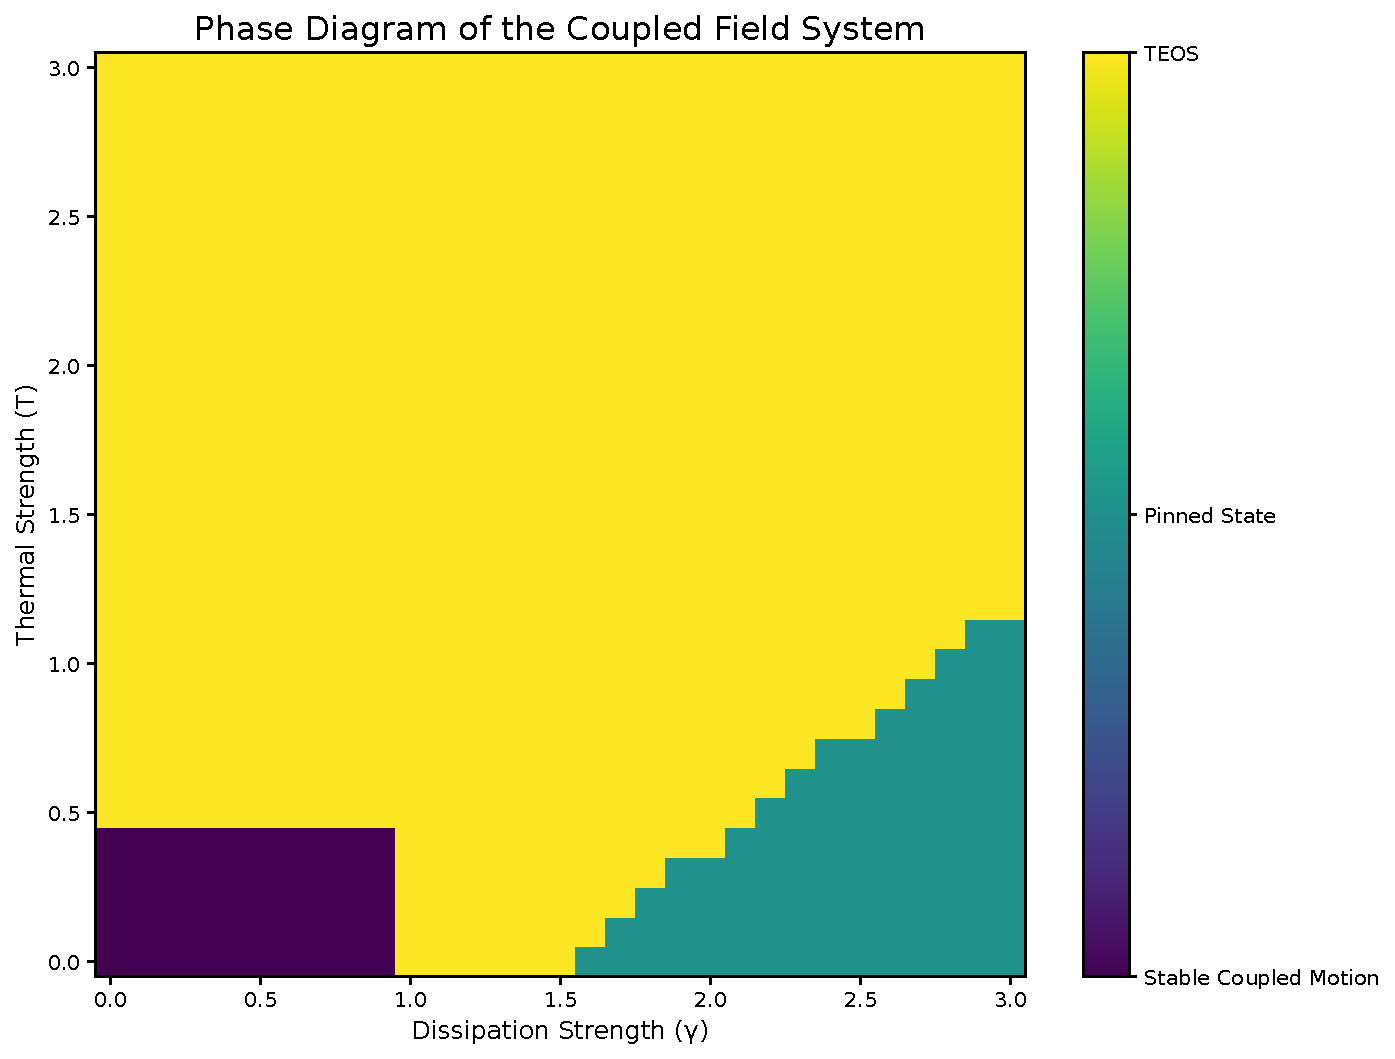
\includegraphics[width=0.8\linewidth]{PhaseDiagram_v1_0.0-3.0_T_0.0-3.0.pdf}
  \caption{散逸強度($\gamma$)と熱的強度($T$)をパラメータとする系の相図。数値シミュレーションにより決定された3つの相(安定結合移動、固定状態、TEOS)の分布を視覚的に示す。}
  \label{fig:phase_diagram}
\end{figure}

\paragraph{強散逸領域におけるSNR}
「強すぎる散逸はSRを抑制する」という物理的知見をさらに補強するため、散逸係数が臨界値($\gamma_c \approx 1.925$)を大きく超える $\gamma=2.5$ の条件下で、追加の数値シミュレーションを行った。その結果を図\ref{fig:strong_damping}に示す。予測通り、以前の研究で$\gamma=1.5$の条件下で観測された顕著なSNRピークは完全に消滅し、SNRは温度に対してほぼ平坦な振る舞いを示す。これは、強散逸領域では熱ゆらぎが系のダイナミクスにほとんど影響を与えられなくなり、SRのメカニズムが機能しなくなることを明確に示している。

\begin{figure}[h!]
  \centering
  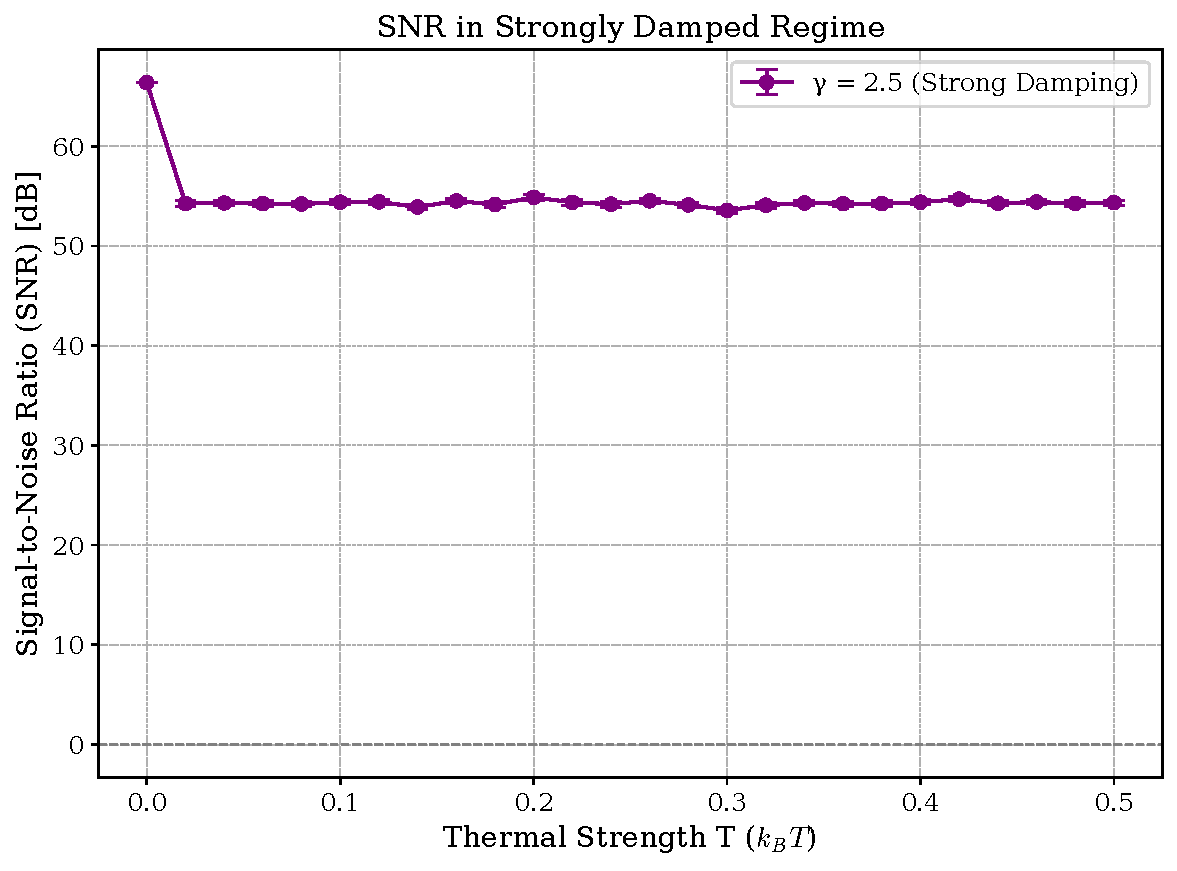
\includegraphics[width=0.8\linewidth]{figA1_strong_damping.pdf}
  \caption{強散逸領域($\gamma=2.5$)におけるSNRの温度依存性。SRピークは完全に抑制されている。}
  \label{fig:strong_damping}
\end{figure}

\paragraph{実効ポテンシャルの妥当性}
本文中で議論した、浅い外部障壁ポテンシャル($A=0.1$)の下で、なぜソリトンが安定に存在できるのかを視覚的に示すため、実効ポテンシャルを図\ref{fig:effective_potential}に示す。ソリトン自身の強い自己束縛相互作用($g=-15.0$)が作る深いポテンシャル井戸($V_{self}$)が、外部障壁($V_{barrier}$)よりも支配的であることが明確にわかる。ソリトンが感じる実効的なポテンシャル($V_{eff}$)は、この自己束縛ポテンシャルによってその形状が決定されており、これによりソリトンは崩壊することなく安定に存在できる。

\begin{figure}[h!]
    \centering
    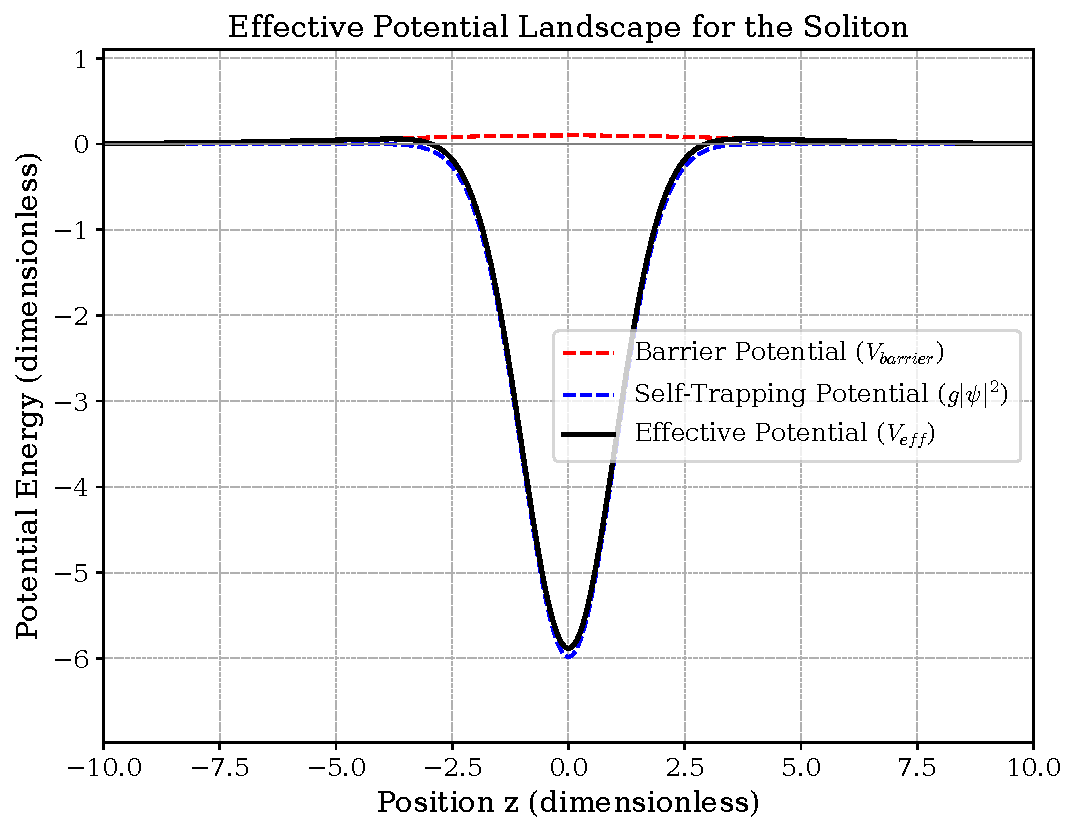
\includegraphics[width=0.8\linewidth]{figA2_effective_potential.pdf}
    \caption{ソリトンが感じる実効ポテンシャルの構造。浅い外部障壁(赤破線)に対し、ソリトン自身の自己束縛(青破線)が作るポテンシャルが支配的であり、安定な実効ポテンシャル(黒実線)を形成している。}
    \label{fig:effective_potential}
\end{figure}

\FloatBarrier
\begin{thebibliography}{99}
\bibitem{feynman} R. P. Feynman, \textit{Phys. Rev.} \textbf{56}, 340 (1939).
\bibitem{ingber} D. E. Ingber, \textit{J. Cell Sci.} \textbf{104}, 613 (1993).
\bibitem{fleck} J. A. Fleck Jr., J. R. Morris, and M. D. Feit, \textit{Appl. Phys.} \textbf{10}, 129 (1976).
\bibitem{kane} C. L. Kane and E. J. Mele, \textit{Phys. Rev. Lett.} \textbf{95}, 146802 (2005).
% --- Added References ---
\bibitem{lindner} B. Lindner, J. García-Ojalvo, A. Neiman, and L. Schimansky-Geier, "Effects of noise in excitable systems", \textit{Physics Reports} \textbf{392}, 321 (2004).
\bibitem{vonneumann} J. von Neumann, "On a Certain Topology for Rings of Operators", \textit{Ann. of Math.} \textbf{37}, 111 (1936).
\bibitem{bratteli} O. Bratteli and D. W. Robinson, "Operator Algebras and Quantum Statistical Mechanics 1", Springer (1987).
\bibitem{benzi} R. Benzi, A. Sutera, and A. Vulpiani, "The mechanism of stochastic resonance", \textit{J. Phys. A: Math. Gen.} \textbf{14}, L453 (1981).
\bibitem{mcnamara} B. McNamara and K. Wiesenfeld, "Theory of stochastic resonance", \textit{Phys. Rev. A} \textbf{39}, 4854 (1989).
\bibitem{gammaitoni} L. Gammaitoni, P. Hänggi, P. Jung, and F. Marchesoni, "Stochastic resonance", \textit{Rev. Mod. Phys.} \textbf{70}, 223 (1998).
\bibitem{bradley} A. S. Bradley, C. W. Gardiner, and M. J. Davis, "The stochastic Gross-Pitaevskii equation: A rigorous formulation for finite-temperature Bose-Einstein condensates", \textit{Phys. Rev. A} \textbf{77}, 033616 (2008).
\end{thebibliography}

\end{document}